%% ----------------------------------------------------------------
%% Thesis.tex -- main
%% ---------------------------------------------------------------- 

\documentclass[a4paper, 10pt, oneside]{memoir}
%% Use the option citeauthor to be able to use citet. The default cite will still work.
\usepackage[citeauthor]{basilea}
\usepackage{stmaryrd}
\newtheorem{theorem}{Theorem}
\newtheorem{definition}[theorem]{Definition}
\newcommand\mytodo[1]{\textbf{\textcolor{magenta}{#1}}}
%\renewcommand\mytodo[1]{} % TODO: this hides all todos

%% ----------------------------------------------------------------

\title				{Mutex Based Potential Heuristics}
\thesistype			{Bachelor thesis}

\department 		{Department of Mathematics and Computer Science}
\faculty			{Natural Science Faculty of the University of Basel}
\research		    {Artificial Intelligence \\ https://ai.dmi.unibas.ch}

\examiner    		{Prof. Dr. Malte Helmert}
\supervisor  		{Salom\'e Eriksson}

\authors     		{Salome M\"uller}
\email				{salo.mueller@unibas.ch}
\immatriculnr		{2017-063-058}

\date				{06. 11. 2020}

% switch here for the german logo to logo-de
\ulogo				{Template/logo-en} 


%% ----------------------------------------------------------------
\begin{document}

% for english use \selectlanguage{english}, for german use \selectlanguage{ngerman}
\selectlanguage{english}

\thesisfront
\maketitle
\pagestyle{thesis}
%% ----------------------------------------------------------------
% % !TEX root = ../Thesis.tex
\chapter{Acknowledgements}\label{ch:acknowledgments}
First, I want to thank Prof. Dr. Malte Helmert for the opportunity of writing my bachelor thesis in the AI group at the University of Basel.
I am very grateful for the support of Dr. Salom\'e Eriksson, who patiently answered all my questions and guided me through this work.
I would like to acknowledge Dr. Florian Pommerening for helping me understand the LP constructor of Fast Downward.


Further, I received a great deal of support and assistance from Lucas Galery K\"aser, as well as from my flatmates.
Thank you all for keeping me nourished.

Last, I want to thank Ada Lovelace, the first programmer there was, for being an inspiration to women in computer science.

Calculations were performed at sciCORE (http://scicore.unibas.ch/) scientific computing center at University of Basel.
%% ----------------------------------------------------------------
%% !TEX root = ../Thesis.tex
\chapter{Abstract}\label{ch:abstract}
\mytodo{
mutexes and disambiguations are an enhancement (verbesserung) but the er too expensive and therefore their coverage is not better.
The additional constraint on the initial state on the other hand is good.
A method which we developed, the additional constraints on random states, are an enhancement too, but not that much
}
%% ----------------------------------------------------------------
\thesistoc
%% ----------------------------------------------------------------
%\thesisnomencl
%% ----------------------------------------------------------------
\thesismain
%! Author = salom
%! Date = 18.09.2020
\chapter{Introduction}\label{ch:introduction}

One dimensional potential heuristics assign a potential, i.e., a numerical value, to each fact of a classical planning problem.
They can be used in a heuristic search, the most common approach to solve such problems.
The potentials are obtained with a Linear Program, which optimizes the potentials according to an optimization function.
Different optimization functions yield different heuristics.
The heuristic value of a state is the sum over the potentials of the fact in this state.

In this thesis, we reproduce the work of~\cite{fivser2020strengthening} who proposed to strengthen potential heuristics with mutexes and disambiguations.
Mutexes are sets of facts, which can never appear together in any reachable state.
They can be used to build disambiguation sets for partial states.
They contain all remaining facts which can be assigned to this partial state, i.e., which are not mutex with any of the facts in the partial state.

As introduced by~\cite{fivser2020strengthening} we use mutexes and disambiguations to build a less restricted Linear Program.
This does lead to better heuristics but the computation is too expensive and slightly less problems are solved.

Next, we use mutexes and disambiguations to strengthen the optimization functions.
This leads to good single and ensemble heuristics, however not more problems can be solved, than with the non-strengthened optimization functions.

Further, we add the additional constraint on the initial state to the constraints of the LP, as~\cite{fivser2020strengthening} proposed.
This does indeed enhance the performance, as the resulting heuristics solve more problems as the same heuristics computed without the additional constraint.

Taking this idea one step further, we add additional constraints on random states.
Therefore, random states are generated with random walks, and constraints gained by optimizing the LP for this states are added.
These additional constraints do not enhance the performance of the resulting heuristics in comparison to the constraint on the initial state.
They are, however, better than using no additional constraint at all, and could be further enhanced.

Last, we compare our results to the evalulation of~\cite{fivser2020strengthening}.
It turns out, that the translation and preprocessing of the planning tasks they use, as well as their way for generating of the potentials, are faster than ours.
%! Author = salom
%! Date = 11.09.2020

\chapter{Background}\label{ch:background}

The goal of this chapter is to define and explain the terminology in this thesis.
For visualization the 8-Tiles problem is used as an example.
This is a classical planning problem, in which 8 tiles are arranged in a 3x3-Grid.
One spot remains empty, the goal is to bring the tiles in a specific order by sliding them around.
% TODO: explain why we do this? what is a classical planning problem?

\section {Planning Tasks}\label{sec:planning-tasks}
In order to solve a classical planning problem with heuristic search it is represented as a \textbf{planning task}.
\citeauthor{fivser2020strengthening} use the finite domain representation (\textbf{FDR}) where $\Pi$ is specified by a tuple $ \Pi = \langle \mathcal{V}, \mathcal{O}, I, G \rangle$~\cite{helmert2009concise}.

$\mathcal{V}$ is a finite set of \textbf{variables}, each of the variables $V\in\mathcal{V}$ has a finite set of \textbf{domains} $\text{dom}(V)$.
For 8-Tiles, the variables could be defined as the 9 fields in the grid ($v_1$ to $v_9$), and their domains hold the values of all tiles and the blank space (1 to 8 and 0 for the blank tile).
A \textbf{fact} $f=\langle V, v\rangle$ consists of a variable $V\in\mathcal{V}$ and one of its values $v\in\text{dom}(V)$.
The fact for tile number 5 being in the first position would be $\langle v_1,5\rangle$.
$\mathcal{F}_V$ is the set of all possible facts of variable $V\in\mathcal{V}$ while $\mathcal{F}$ is the set of all facts of this problem.

A \textbf{partial state} $p$ of size $t$ contains $t$ facts of $t$ different variables, i.e., it is the variable assignment over the variables $\text{vars}(p)\subseteq\mathcal{V}$ with $|\text{vars}(p)|=t$.
$p[V]$ is the value assigned to $V$ in $p$.
In other words, $p=\{\langle V, p[v] \rangle | V\in\text{vars}(p)\}$.
A \textbf{state} $s$ is not partial, if all variables are assigned, i.e., $\text{vars}(s)=\mathcal{V}$.
It \textbf{extends} the partial state $p\subseteq s$, if $s[v] = p[v]$ for all $v \in\text{vars}(p)$.
The partial state $p = \{v_1\mapsto0, v_2\mapsto1\}$ represents all states where the first grid in the field of the 8-Tiles puzzle is the blank space while tile number one lies in the second field.

$I$ is the \textbf{initial state}, in 8-Tiles this is some specific random order of the tiles.
$G$ is a partial state representing the \textbf{goal}. $s$ is a \textbf{goal state}, if it is an extension of $G$.
In 8-Tiles it is one specific order of the tiles e.g. sorted by number:
$s = \{v_1\mapsto1, v_2\mapsto2, v_3\mapsto3, v_4\mapsto4, v_5\mapsto5, v_6\mapsto6, v_7\mapsto7, v_8\mapsto8, v_9\mapsto0\}$.

$\mathcal{O}$ is a finite set of \textbf{operators}.
Each $o\in\mathcal{O}$ has a precondition $\text{pre}(o)$ and an effect $\text{eff}(o)$ which are both partial states over $\mathcal{V}$, and a cost $\text{c}(o)\in\mathbb{R}^+_0$.

The operator $o$ is \textbf{applicable} in state $s$ iff $\text{pre}(o)\subseteq s$, the \textbf{resulting state} is $o\llbracket s\rrbracket$.
$o\llbracket s\rrbracket[v] = \text{eff}(o)[v]$ holds for all $v\in \text{eff}(o)$ in resulting state $o\llbracket s\rrbracket$, while $o\llbracket s\rrbracket[v]=s[v]$ for all $v\notin \text{eff}(o)$. \mytodo{reformulate.}
In 8-Tiles the operators encode the movement of one tile to the blank space.
The precondition assures that the tile is next to the blank space, the effect swaps the values of the corresponding two variables, while all other tiles remain at the same position.

In order to reach the goal multiple operators need to be applied in a specific order.
A sequence of operators $\pi=\langle o_1,\dots, o_n\rangle$ is called a path, $\pi\llbracket s\rrbracket = s_n$.
$\pi$ is a \textbf{s-plan}, if $\pi$ is applicable in $s$ and $\pi\llbracket s\rrbracket$ is a an extension of $G$ and therefore a goal state.
If it has minimal cost among all s-plans it is called \textbf{optimal}.

The set $\mathcal{R}$ is defined as the set of all \textbf{reachable} states.
A state $s$ is reachable, if a plan $\pi$ is applicable in $I$ such that $\pi\llbracket I\rrbracket = s$.
An operator $o$ is reachable, if it is applicable in a reachable state.
A state $s$ is a \textbf{dead-end state} if it does not extend the goal state, and no s-plan exists.

%TODO: introduce transition normal form?

\section{Heuristics}\label{sec:heuristics}
A \textbf{heuristic} $h:\mathcal{R} \rightarrow \mathbb{R} \cup \{\infty\} $ estimates the cost of the optimal plan for a state $s$.
The problem of 8-Tiles has uinform cost, as sliding a tile always costs the same, i.e. 1, and there are no other operators.
Therefore, the cost of a s-plan of any state which is not a dead-end equals the amount tiles, which need to be slid in the plan.
The \textbf{optimal heuristic} $h^*(s)$ maps each state $s$  to its actual optimal cost, or to $\infty$ if it is a dead-end state.
We aim to approach this heuristic.

This thesis uses heuristics in the forward heuristic search where unreachable states are never expanded.
Therefore they are defined over $\mathcal{R}$ instead of over all states and the above defined rules hold for reachable states only.

A heuristic is \textbf{admissible}, if it never overestimates the optimal heuristic, i.e., $h(s)\leq h^*(s)$.
It is \textbf{goal-aware} iff $h(s)\leq 0$ for all reachable goal states, i.e., it recognizes a goal sate as such.
Further, it is \textbf{consistent} iff $h(s)\leq h(o\llbracket s\rrbracket)+c(o)$.
This rule assures, that the heuristic of the successor of a state is not a a lot lower than the heuristic of the state itself.

A heuristic which is goal aware and consistent is also admissible.

One class of heuristics are potential heuristics which assign a potential to each possible fact of the planning task.
\begin{definition}
    Let $\Pi$ denote a planning task with facts $\mathcal{F}$.
    A \textbf{potential function} is a function $\mathtt{P}:\mathcal{F}\mapsto\mathbb{R}$.
    A \textbf{potential heuristic} for $\mathtt{P}$ maps each state $s\in\mathcal{R}$ to the sum of potentials of facts in $s$, i.e., $h^\mathtt{P}(s)=\sum_{f\in s}P(f)$.
\end{definition}

Potential heuristics are goal-aware, consistent and admissible~\cite{fivser2020strengthening}.
The potentials themselves are obtained through optimization which will be further analyzed in Chapter~\ref{ch:strengthening-potential-heuristics}.

One further approach is \textbf{ensemble heuristics}.
Instead of only one heuristic, this approach uses multiple heuristics and chooses the highest value as heuristic value for each state.

\section{Mutexes and Disambiguations}\label{sec:mutexes-and-disambiguations}
Mutex means, that two or more things mutually exclude each other.

\begin{definition}
    Let $\Pi$ denote a planning task with facts $\mathcal{F}$.
    A set of facts $\mathcal{M}\subseteq \mathcal{F}$ is a \textbf{mutex} if $\mathcal{M}\nsubseteq s$ for every reachable state $s\in\mathcal{R}$
\end{definition}

Facts are a mutex if they never appear together in any reachable state.
If a partial state $p$ in 8-Tiles holds $p[v_3]=1$, then tile one may not be in any other spot of the grid, i.e., the fact $\langle v_3, 1\rangle$ is mutex with all
other facts $\langle v, 1\rangle$ with $v\in \mathcal{V}\setminus \{v_3\}$.

\begin{definition}
    Let $\Pi$ denote a planning task with variables $\mathcal{V}$ and facts $\mathcal{F}$.
    A set of sets of facts $\mathcal{M}\subseteq 2^{\mathcal{F}}$ is called a \textbf{mutex-set} if the following hold:
    (a) every $M\in\mathcal{M}$ is a mutex;
    and (b) for every $M\in\mathcal{M}$ and every $f\in\mathcal{F}$ it holds that $M\cup\{f\}\in\mathcal{M}$;
    and (c) for every variable $V\in\mathcal{V}$ and every pair of facts $f, f'\in\mathcal{F}_V$, $f\neq f'$, it holds
    that $\{f,f'\}\in\mathcal{M}$.
\end{definition}

We can say that $s\in\mathcal{M}$ if $s$ contains a subset of facts which are a mutex.

Mutexes can be used to derive disambiguations.
\begin{definition}
    Let $\Pi$ denote a planning task with facts $\mathcal{F}$ and variables $\mathcal{V}$, let $V\in\mathcal{V}$ denote
    a variable, and let $p$ denote a partial state.
    A set of facts $F\subseteq\mathcal{F}_V$ is called a \textbf{disambiguation} of $V$ for $p$ if for every reachable state
    $s\in\mathcal{R}$ such that $p\subseteq s$ it holds that $F\cap s\neq\emptyset$ (i.e., $\langle V,s[V]\rangle\in F$).
\end{definition}

The disambiguation of a variable $V$ for a partial state $p$ is the set of facts $F\in\mathcal{F}_V$ which occur in all reachable extended states of $p$.
This means, that each fact of $V$ which is not in $F$ is a mutex with $p$.
If $F$ contains exactly one fact then $p$ can be safely extended with that fact, as it is the only non-dead-end extension of the state.
If $F$ is the empty set every extended state of $p$ is a dead-end.
This knowledge can be used to prune operators $o$ for which $p\subseteq\text{pre}(o)$ and unreachable states $s\subseteq p$.
If the goal state $G$ is one of this states, the problem is unsolvable.

If a partial state $s$ of the 8-Tiles problem holds $p[v_3] = 1$ and $p[v_2] = 1$, then it is a dead-end, as these facts are a mutex.
If $p = \{v_1\mapsto1, v_2\mapsto2, v_3\mapsto3, v_4\mapsto4, v_5\mapsto5, v_6\mapsto6, v_7\mapsto7, v_8\mapsto8\}$ then $p$ is not a dead-end and $v_9$ can safely be assigned with $0$, as it is the only fact in $\mathcal{F}_{v_9}$ which does not form a mutex with any of the already assigned facts.

The set $\mathcal{M}_p=\{f|f\in\mathcal{F}, p\cup\{f\}\in\mathcal{M}\}$ is the set of facts which are mutex with $p$.
All facts of a variable $f\in\mathcal{F}_V$ not contained in $\mathcal{M}_p$ build the disambiguation $F$ of $V$ for $p$.
In~\ref{ch:strengthening-potential-heuristics} we will use this to improve potential heuristics by narrowing down possible extensions of partial states.



%! Author = salom
%! Date = 11.09.2020

\chapter{Strengthening Potential Heuristics}\label{ch:strengthening-potential-heuristics}

\citeauthor{fivser2020strengthening} propose a method to improve potential heuristics with mutexes and disambiguations.
This chapter contains the changes which are required to do so, regarding the transformation of a planning task into TNF and the adaption of the optimization functions.
It shows how the equations which were later implemented (Section~\nameref{sec:implementation}) are derived.

\section{Potential Heuristics}\label{sec:potential-heuristics}

When~\citeauthor{pommerening2015non} first introduced potential heuristics, they showed that two inequalities are sufficient to proof admissibility.

\begin{theorem}
    \label{theorem:theorem 5} % Theorem 6
    Let $\Pi = \langle \mathcal{V}, \mathcal{O}, I, G \rangle$ denote a planning task, $\mathtt{P}$ a
    potential function, and for every operator $o\in\mathcal{O}$, let
    $\mathrm{pre}^*(o)=\{\langle V, \mathrm{pre}(o)[V]\rangle |V\in \mathrm{vars(pre}(o))\cap\mathrm{vars(eff}(o))\}$ and
    $\mathrm{vars}^*(o)=\mathrm{vars(eff}(o))\setminus\mathrm{vars(pre}(o))$. If
    \begin{equation}\sum_{f\in G}\mathtt{P}(f)+\sum_{V\in\mathcal{V}\setminus\mathrm{vars}(G)}\max_{f\in\mathcal{F}_V}\mathtt{P}(f)\leq0\label{eq:1}\end{equation}
    and for every operator $o\in\mathcal{O}$ it holds that
    \begin{equation}sum_{f\in\mathrm{pre}^*(o)}\mathtt{P}(f)+\sum_{V\in\mathrm{vars}^*(o)}\max_{f\in\mathcal{F}_V}\mathtt{P}(f)-\sum_{f\in\mathrm{eff}(o)}\mathtt{P}(f)\leq c(o)\label{eq:2}\end{equation}
    then the potential heuristic for $\mathtt{P}$ is admissible.
\end{theorem}


Eq.~\eqref{eq:1} of the Theorem~\ref{theorem:theorem 5} assures goal-awareness of the potential heuristic.
As all variables are assigned in the goal state, the potential of one fact per variable has to be summed up.
For the variables $v\in\text{vars}(G)$ we can simply use the potentials of their respective facts.
Meanwhile we assume the worst case for the other variables, by using the maximal potential over their facts, as we do not know what fact they are assigned.

Eq.~\eqref{eq:2} assures consistency.
Recall the general heuristics consistency equation $h(s)\leq h(o\llbracket s\rrbracket)+\text{c}(o)$.
It can be rewritten as $h(s)-h(o\llbracket s\rrbracket)\leq\text{c}(o)$.
As the facts which do not occur in the effect are the same in both $s$ and $o\llbracket s\rrbracket$ we can leave them aside. % da substraktion
For $s$ we know what facts of the variables of the preconditions are assigned and sum the potentials of the facts which are in the effect as well.
For the variables which are in the effect but not in the precondition we proceed similarly to ~\eqref{eq:1}, as we do not know their values.
The potentials of the facts in the effect can be used without modification for  $o\llbracket s\rrbracket$.

The advantage of these equations is that they are not state-dependent, even though they do not tell us explicitly what the potentials should be.
However, they can be used as the constraints for a linear program, the solution of which is a potential function that forms an admissible potential heuristic.
More about this in Section~\ref{sec:transition-normal-form}.

\subsection{Generalization with Mutexes}\label{subsec:pot-generalize-with-mutexes}
Mutexes can be used to reduce the domain of variables, which are not yet assigned in a partial state $p$.
This property is very helpful, as it minimizes the amount of facts which are candidates for the not assigned variables in Equations~\eqref{eq:1} and~\eqref{eq:2} of Theorem~\ref{theorem:theorem 5}.

\mytodo{make this algorithm look a little nicer\ldots}
\begin{algorithm}[H]
    \caption{Multi-fact fixpoint disambiguation.}
    \label{alg:multi-fact}
    \begin{algorithmic}[1] % The number tells where the line numbering should start
        \Require A planning task $\Pi$ with variables $\mathcal{V}$ and facts $F$, a partial state $p$, and a mutex-set $\mathcal{M}$.
        \Ensure A set of disambiguations $\mathcal{D}_p$ of all variables $\mathcal{V}$ for $p$.

        \State $D_v\leftarrow F_V$ for every $V\in\mathcal{V}$\;
        \State $A\leftarrow \mathcal{M}_p$\;
        \State change $\leftarrow$ True\;
        \While{change\;}
        \State change $\leftarrow$ False\;
        \ForAll{$V\in\mathcal{V}$}
        \If{$D_V\setminus A\neq D_V $}
        \State $D_V\leftarrow D_V\setminus A$\;
        \State $A\leftarrow A\cup \bigcap_{f\in D_V}\mathcal{M}_{p\cup \{f\}} $\; \label{lst:line:A}
        \State change $\leftarrow$ True\;
        \EndIf
        \EndFor
        \EndWhile
        \State $\mathcal{D}_p\leftarrow\{D_V|V\in\mathcal{V}\}$\;
    \end{algorithmic}
\end{algorithm}

At the beginning, the set $D_V$ contains all possible values for the variable $V\in\mathcal{V}$, while $A$ contains all facts which are a mutex with any fact in $p$.
In each iteration of the while-loop, all $f=\langle v, V\rangle$ which are in $A$ and in $D_V$ are removed from the corresponding $D_V$.
On line~\ref{lst:line:A}, $A$ is extended with all facts that form a mutex with all facts remaining in $D_V$, i.e., which are a mutex with $p\cup\{f\}$ for all $f\in D_V$.

In conclusion, after applying mutli-fact fixpoint disambiguation $p$ can be extended with any fact in $\mathcal{D}_p$ without reaching a dead-end state.
If any $D_V\in\mathcal{D}_p$ is empty, then $p$ is already a dead-end itself.

This algorithm is used for several applications during the remainder of this chapter.
In this section, it can be used to generalize Theorem~\ref{theorem:theorem 5} by the following theorem.

\begin{theorem}
    \label{theorem:7}
    Let $\Pi = \langle \mathcal{V}, \mathcal{O}, I, G \rangle$ denote a planning task with facts $\mathcal{F}$, and let $\mathtt{P}$ denote a potential function, and
    \begin{enumerate}[(i)]
        \item for every variable $V\in\mathcal{V}$, let $G_V\subseteq\mathcal{F}_V$ denote a disambiguation of $V$ for $G$ s.t. $|G_V|\geq1$, and
        \item for every operator $o\in\mathcal{O}$ and every variable $V\in\mathrm{vars(eff}(o))$, let $E^o_V\subseteq\mathcal{F}_V $ denote a disambiguation of $V$ for $\mathrm{pre}(o)$ s.t. $|E^o_V|\geq1$.
    \end{enumerate}

    If
    \begin{equation}\sum_{V\in\mathcal{V}}\max_{f\in G_V}\mathtt{P}(f)\leq0\label{eq:3}\end{equation}
    and for every operator $o\in\mathcal{O}$ it holds that
    \begin{equation}\sum_{V\in\mathrm{vars(eff}(o))}\max_{f\in E^o_V}\mathtt{P}(f) - \sum_{f\in\mathrm{eff}(o)}\mathtt{P}(f)\leq\mathrm{c}(o)\label{eq:4}\end{equation}
    then the potential heuristic $\mathtt{P}$ is admissible.
\end{theorem}

\citeauthor{fivser2020strengthening} prove the theorem by showing that Equations~\eqref{eq:3} and~\eqref{eq:4} are generalizations of Equations~\eqref{eq:1} and~\eqref{eq:2}, respectively.

The disambiguation $G_V$ equals $D_V\in\mathcal{D}_G$ with $V\in\mathcal{V}$, which is generated by applying Algorithm~\autoref{alg:multi-fact} on the goal state.
If it is empty for any of the variables, then the problem is unsolvable, as the goal contains a mutex and is therefore not a reachable state.
$E_V^o$ is equal to $D_V\in\mathcal{D}_{\text{pre}(o)}$.
$o$ is not applicable in any (partial) state if $E^o_V$ is empty for any  $V\in\text{vars(eff}(o))$.

To show the reader why this property is useful in practice, we first introduce the Transition Normal Form.

\section{Transition Normal Form}\label{sec:transition-normal-form}
Planning tasks can be in Transition Normal Form (TNF).
A planning task in TNF has a fully defined goal ($\text{vars}(G)=\mathcal{V}$) and all variables of the effect are also in the precondition for each operator $o\in\mathcal{O}$ ($\text{vars(pre}(o)) = \text{vars(eff}(o))$).
These properties are essential to form the Linear Program, which we will do in the next section.
Any planing task  $\Pi = \langle \mathcal{V}, \mathcal{O}, I, G \rangle$ can be transformed into TNF with the following rules cited from~\citeauthor{fivser2020strengthening}:
\begin{itemize}
    \item Add a fresh value $U$ to the domain of every variable.
    \item For every variable $V\in\mathcal{V}$ and every fact $f\in\mathcal{F}_V$, $f\neq\langle V,U\rangle$, add a new \textit{forgetting} operator $o_f$ with $\text{pre}(o_f)=\{f\}$ and $\text{eff}(o_f)=\{\langle V,U\rangle\}$ and the cost $\text{c}(o_f)=0$.
    \item For every operator $o\in\mathcal{O}$ and every variable $V\in\mathcal{V}$:
    \begin{itemize}
        \item If $V\in\text{vars(pre}(o))$ and $V\notin\text{vars(eff}(o))$, then add $\langle V,\text{pre}(o)[V]\rangle$ to $\text{eff}(o)$.
        \item If $V\in\text{vars(eff}(o))$ and $V\notin\text{vars(pre}(o))$, then add $\langle V,U\rangle$ to $\text{pre}(o)$.
    \end{itemize}
    \item For every $V\in\mathcal{V}\setminus\text{vars}(G)$ add $\langle V,U\rangle$ to $G$.
\end{itemize}

Each Variable $V\in\mathcal{V}$ gets a new value $U$ in its domain, which can be seen as a sort of placeholder.
The fact $\langle V,U\rangle$ can be assigned with cost 0, as the forgetting operator $o_f$ which assigns it has no cost, regardless of the current state and especially the current assignment of $V$.
The next point is to assure that for each operator the variables which are in the precondition are also in the effect.

If $V$ is present in the preconditions of an operator $o\in\mathcal{O}$ but not in the effect, then we can simply add the variable and the value it is already assigned to the effect.
This is a formal change, but does not change the effect of the operator at all, as it would not have changed this fact anyway.

The case of an operator $o\in\mathcal{O}$, where $V$ is in the effect but not in the precondition, is a little more complicated.
Here, the precondition is changed such that it contains also the fact $\langle V, U\rangle$.
If $o$ was applicable in $s$ before, then, after transforming the plan into TNF, the corresponding $o_f$ needs to be applied beforehand in order to forget the value of $V$.
This change of the variable is insignificant, as the value then gets changed by applying the operator anyways.

Last, all variables which were not included in the partial state $G$ need to be added into it.
If they are assigned the fresh value $U$, then the goal state can be reached from every state which expanded it before.
Without creating more cost, the values of all unimportant variables are changed to the fresh value.
The compilation into TNF can produce a plan twice the size of the original task in worst case~\cite{seipp2015new}.

\subsection{Generalization with Mutexes}\label{subsec:tnf-generalize-with-mutexes}
Similar to Section~\ref{subsec:pot-generalize-with-mutexes}, these rules can be generalized with disambiguations.
Therefore, to replace $U$ we introduce the fresh values $U_{G_V}$ and $U_{E^o_V}$.
Instead of adding forgetting operators from every fact in every $V\in\mathcal{V}$, we use the disambiguation sets $G_V$ and $E_V^o$.

\begin{itemize}
    \item Add fresh value $U_{G_V}$ to the domain of every $V\in\mathcal{V}$.
    \item For every variable $V\in\mathcal{V}$ and every fact $f\in G_V$, $f\neq\langle V,U_{G_V}\rangle$, add new \textit{forgetting} operators $o_{f_G}$ with $\text{pre}(o_{f_G})=\{f\}$ and $\text{eff}(o_{f_G})=\{\langle V,U_{G_V}\rangle\}$ and the cost $\text{c}(o_{f_G})=0$.
    \item For every $V\in\mathcal{V}\setminus\text{vars}(G)$ add $\langle V,U_{G_V}\rangle$ to $G$.
    \item For every operator $o\in\mathcal{O}$ add fresh value $U_{E^o_V}$ to the domain of every $V\in\mathcal{V}$:
    \begin{itemize}
        \item If $V\in\text{vars(pre}(o))$ and $V\notin\text{vars(eff}(o))$, then add $\langle V,\text{pre}(o)[V]\rangle$ to $\text{eff}(o)$.
        \item If $V\in\text{vars(eff}(o))$ and $V\notin\text{vars(pre}(o))$, then add $\langle V,U_{E^o_V}\rangle$ to $\text{pre}(o)$.
    \end{itemize}
    \item For every variable $V\in\mathcal{V}$, every operator$o\in\mathcal{O}$ and every fact $f\in E_V^o$, $f\neq\langle V,U_{E^o_V}\rangle$, add new forgetting operators $o_{f,o}$ with $\text{pre}(o_{f,o})=\{f\}$ and $\text{eff}(o_{f,o})=\{\langle V,U_{E^o_V}\rangle\}$ and the cost $\text{c}(o_{f,o})=0$.
\end{itemize}

For the goal state, forgetting operators are only created for the facts in $F_V$ which are not a mutex with any $f\in G$ for every $V\notin\text{vars}(G)$.
Similarly, facts in $F_V$ which are a mutex with any $f\in\text{pre}(o)$ are not taken into account for all $o\in\mathcal{O}$ and every $V\in\text{vars(eff}(o))$.
This creates at most $|\mathcal{O}|*|\mathcal{V}|$ $U_{E_V^o}$ and $|\mathcal{V}|$ $U_{G_V}$ and the amount of forgetting operators is in the worst case the same, multiplied with the sum of the cardinalities of the domains of all $V\in\mathcal{V}$.
In practice,~\citeauthor{fivser2020strengthening} show that the transformation with disambiguations is never bigger than without disambiguations.

\section{Linear Program}\label{sec:linear-programm}
The formulas and rules which were defined in the previous two sections can now be used to form a Linear Program (LP).

An LP consists of LP-variables which are constrained by multiple inequalities (constraints) and which are part of an optimization function.
An LP-solver then assigns each LP-variable a value, such that all constraints are satisfied and the optimization function is optimized.
We will look at different optimization functions in the next section (\ref{sec:optimization}).

\begin{definition}
    \label{definition:LP}
    Let $f$ be a solution to the following LP:

    Maximize $\mathrm{opt}$ subject to $\sum_{V\in\mathcal{V}}\mathtt{P}_{\langle V, s[V]\rangle}\leq0$ and
    $\sum_{V\in\mathrm{vars(eff}(o))}(\mathtt{P}_{\langle V, \mathrm{pre}(o)[V]\rangle}-\mathtt{P}_{\langle V, \mathrm{eff}(o)[V]\rangle})\newline\leq\mathrm{c}(o)$
    for all $o\in\mathcal{O}$, where the objective function $\mathrm{opt}$ can be chosen arbitrarily.

    Then the function $\mathrm{pot}_{\mathrm{opt}}(\langle V,v\rangle)=f(\mathtt{P}_{\langle V,v\rangle})$ is the {\normalfont potential function optimized for $\mathrm{opt}$} and $h^{\mathtt{p}}$ is the {\normalfont potential heuristic optimized for $\mathrm{opt}$}.
\end{definition}

In order to find a potential heuristic, the LP-variables are the potentials of the facts, $P(f)$.
Further we define the constraints as Equation~\eqref{eq:3} for the goal state and Equations~\eqref{eq:4} for every operator.
Since these two formulas assure admissibility, any solution of the LP builds an admissible $h^\mathtt{p}$.
We introduce the the LP-variables $X_f=\mathtt{P}(f)$ for every $f\in\mathcal{F}$ and $M_{G_V}$ and $M_{E^o_V}$ corresponding to $U_{G_V}$ and $U_{E_V^o}$, respectively, with the constraint that $X_f\leq M_{G_V}$ for every $f\in G_V$ and $X_f\leq M_{E^o_V}$ for every $f\in E^o_V$.
This gives the constraints
\begin{equation}\sum_{f\in G}X_f+\sum_{V\in\mathcal{V}\setminus\text{vars}(G)}M_{G_V}\leq0\end{equation}
and
\begin{equation}\sum_{f\in\text{pre}^*(o)}X_f+\sum_{V\in\text{vars}^*(o)}M_{E^o_V}-\sum_{f\in\text{eff}(o)}X_f\leq c(o)\end{equation}
which are coherent to the formulas in Definition~\ref{definition:LP} (\citeauthor{pommerening2015non}).
$M_{G_V}$ and $M_{E^o_V}$ correspond to $U_{G_V}$ and $U_{E_V^o}$, respectively, since these are the facts which are assigned if a variable is not defined in the goal state or in a precondition of an operator.

The solution of the LP might differ vastly depending on the used optimization function.
We will look at multiple different possibilities for optimization functions.

\section{Optimization Functions}\label{sec:optimization}
An optimization function $\mathrm{opt}$ is a linear combination of the LP-variables.
In our case, the goal is to have best possible heuristic value for as many states as possible.
Using different optimization functions optimizes different aspects of a heuristic.
The perfect heuristic would be achieved, if we optimized the potentials for each single state, but this is computationally too expensive.

In the first proposal for potential heuristics from~\citeauthor{pommerening2015non}, the optimization for the initial state was used,
\begin{equation}\mathrm{opt}_I=\sum_{f\in I}\mathtt{P}(f).\label{eq:initial-state}\end{equation}
It optimizes the heuristic value for the initial state.
The drawback of is that facts which do not appear in the initial state are not taken into account.

Alternatively, we could optimize the potentials for all reachable states, with the all-states-potentials optimization function:
\begin{equation}\mathrm{opt}_\mathcal{R} = \frac{1}{|\mathcal{R}|}\sum_{s\in\mathcal{R}}\sum_{f\in s}\mathtt{P}(f).\label{eq:all-states}\end{equation}

It calculates the weighted sum of all facts, i.e., it multiplies the potential of a fact with the amount of reachable states containing this fact and normalizes it with the total amount of reachable states.
The potentials generated with this optimization function would result in the heuristic with the maximal average heuristic value over all reachable states.
Unfortunately, calculating this is, again, computationally expensive or even infeasible, if the planning task and therefore the size of $\mathcal{R}$ are big, as the set of reachable states is not known.
To avoid this, we could sample some states $S\subseteq\mathcal{R}$, and calculate Equation~\eqref{eq:all-states} over these states, instead of $\mathcal{R}$:
\begin{equation} \mathrm{opt}_\mathcal{\hat{S}}=\frac{1}{|\mathcal{S}|}\sum_{s\in\mathcal{S}}\sum_{f\in s} \mathrm{P}(f).\label{eq:uniform-opt}\end{equation}

The optimization function could also assume uniform distribution and give all facts the same weight.
Instead of going over all facts of all states, we would sum over the domains of all variables:
\begin{equation} \mathrm{opt}_\mathcal{S}=\sum_{\langle V,v \rangle\in\mathcal{F}}\frac{1}{|\mathrm{dom}(V)}\mathtt{P}(\langle V,v \rangle).\end{equation}

These two approaches for the all-states-potential optimization function can be strengthened with mutexes and disambiguations, which we will describe in the next sections.

\subsection{Strengthening All State Potentials}\label{subsec:strengthening-all-state-potential}
To estimate the amount of reachable states containing $f=\langle V,v \rangle$, we will calculate the upper bound of these states, and try to lower it for each $f\in\mathcal{F}$.
The product of the domains of all variables except $V$, since $V$ is already assigned, is the total amount of states, reachable and non-reachable, which contain $f$.
With Algorithm~\ref{alg:multi-fact} from Section~\ref{subsec:pot-generalize-with-mutexes} we can remove all facts from all domains which are mutex with $f$.
These facts could never be assigned in any reachable state containing $f$.
Therefore, the product over all domains in the resulting disambiguation set is again an upper bound of appearances of $f$.

This holds not only for a single fact, but can be applied to estimate the appearances of any partial state $p$.
As the product of all domains in the disambiguation set is taken, the value is zero, if $p$ is a mutex itself.

If we define $\mathcal{M}$ as the superset of all mutexes and $\mathcal{M}_p$ as the set of all facts which form a mutex with patial state $p$, then an upper bound for the amount of reachable states of size $k$ containing $f$ is

\begin{equation}
    \mathcal{C}_f^k(\mathcal{M}) = \sum_{p\in\mathcal{P}_k^{\{f\}}}\prod_{V\in\mathcal{V}} |F_V\setminus\mathcal{M}_p|
.\label{eq:ckf}\end{equation}

The Equation has the constraint to only extend states to size $k$, as it would get computationally too expensive to compute all reachable states for which $f$ holds.

We will now use Equation~\eqref{eq:ckf} to calculate the weights for the potential of each $f\in\mathcal{F}$ and form the following optimization function:

\begin{equation}
    \mathrm{opt}^k_\mathcal{M}=\sum_{f=\langle V,v \rangle\in\mathcal{F}}\frac{\mathcal{C}_f^k(\mathcal{M})}{\sum_{f'\in\mathcal{F}_V}\mathcal{C}_{f'}^k(\mathcal{M})}\mathtt{P}(f).
    \label{eq:opt1}
\end{equation}

The result is a modification of $\mathrm{opt}_{\hat{S}}$ (Eq.~\eqref{eq:uniform-opt}) that des not assume uniformly distributed facts.
Each fact is weighted according to its estimated appearance in all reachable states of size $k$ in relation to the other facts of the corresponding variable.
The sum of the weights for all facts of one variable is 1.
We can use this not only as a single heuristic, but also in ensemble heuristics as we will show in the next section.

\subsection{Strengthening Conditioned Ensemble Potentials}\label{subsec:strengthening-conditioned-ensemble}
If we divide $\mathcal{R}$ into multiple subsets $S_i\subset\mathcal{R}$, with $i=1,\dots,n$ and $S_1\cup\dots\cup S_n=\mathcal{R}$, the solution of the LP with optimization function $\mathrm{opt}_{\hat{S}_i}$ gives better heuristic values for the states in $S_i$ than $\mathrm{opt}_\mathcal{R}$.
If we calculate the potentials for the optimization of all $S_i$, the resulting heuristics can be used as ensemble heuristics.
This gives a result which lies somewhere between the all-states-potential heuristic and calculating the potentials for each individual state.

We will choose $S_i$ as the states extending one particular partial state $t$, and use the potentials generated with an adjusted $\mathrm{opt}^k_\mathcal{M}$ as one of multiple ensemble heuristics.
For this we adapt Equation~\eqref{eq:ckf}, such that it counts how many reachable states of size $|t| + k$ extend $t$:
\begin{equation}
    \mathcal{K}^k_f(\mathcal{M}, t) = \sum_{p\in\mathcal{P}^{t\cup\{f\}}_{|t|+k}}\prod_{V\in\mathcal{V}}|\mathcal{F}\setminus\mathcal{M}_p|.
\end{equation}

The corresponding optimization function uses the weights calculated with $\mathcal{K}^k_f(\mathcal{M}, t)$,
\begin{equation}
    \mathrm{opt}^{t,k}_\mathcal{M}=\sum_{f=\langle V,v \rangle\in\mathcal{F}}\frac{\mathcal{K}^k_f(\mathcal{M}, t)}{\sum_{f'\in\mathcal{F}_V}\mathcal{K}^k_f(\mathcal{M}, t)}\mathtt{P}(f).
    \label{eq:opt2}
\end{equation}

For this thesis, the partial states $t$ were sampled uniformly at random, as did~\citeauthor{fivser2020strengthening}.
Future research could be to investigate other ways to choose them.

\subsection{Adding Constraint on Initial State}\label{subsec:adding-constraint-on-initial-state}
Both $\mathrm{opt}^k_\mathcal{M}$ and $\mathrm{opt}^{t,k}_\mathcal{M}$ optimize the potentials in regard of the entire reachable state space.
However, the importance of states may vary strongly, depending on where we start and what path is taken from there towards the goal.
For example, a planning task with multiple goal states may have smaller heuristic values, even though the constraints enforce goal-awareness.
This is why we now look at a third approach which gives the initial state more weight and adds the constraint  \begin{equation}\sum_{f\in I}\mathtt{P}(f)=h^\mathtt{P}_I (I)\end{equation} to the Linear Program, where $h^\mathtt{P}_I$ denotes the potential heuristic optimized for the initial state (Eq.~\eqref{eq:initial-state}).
By calculating the potentials for this heuristic first and then taking it into account for the actual potentials, we force the solver to find potentials which guarantee high heuristic values for the initial state.
This approach can be combined with all previously discussed optimization functions.

\section{Implementation}\label{sec:implementation}
Our implementation of mutex based potential heuristics is embedded in the planning system Fast Downward and written in C++.

We first implemented Algorithm~\ref{alg:multi-fact}, which uses the Fast Downward hm-heuristic with $m=2$ to build a mutex table.
The computation of the hm-heuristic in Fast Downward is very slow.
Therefore we implemented a new generator for the mutex table, which has a very similar approach to the hm-heuristic, but which is optimized for finding mutexes.
We show that it is faster in Chapter~\ref{ch:evaluation}

Fast Downward has a potential optimizer, which initializes and constructs an LP-solver.
We implemented a new LP-constructor which builds the constraints according to Equations~\eqref{eq:3} and~\eqref{eq:4}.
For both the non-mutex and the mutex constructor, we added the option to use the additional constraint on the initial state.

Next, we implemented the optimization function $\mathrm{opt}^k_\mathcal{M}$.
All partial states of cardinality one ($p_f = \{f\}$ for all $f\in\mathcal{F}$) are generated, and then recursively all partial states of size $k$ extending $p_f$ are created, using the disambiguation set $\mathcal{D}_{p_f}$.
Even for small tasks the amount of extended states can grow very fast.
For memory efficiency partial states are implemented as maps, containing the assigned facts only.
Using these states, we calculate the weight of each fact with $\mathcal{C}_f^k(\mathcal{M})$.
The weights are stored as vectors and passed to the potential optimizer, which uses them to generate the optimization function.

The optimization function $\mathrm{opt}^{t,k}_\mathcal{M}$ was implemented implicitly.
As all former mentioned methods can handle partial states of a cardinalities $\geq 1$, only one new method was needed.
It generates $n$ mutex based potential heuristics, each of which uses a random state of size $t$.
With each of these we perform the same procedure as above with $p_f$.

Running Fast Downward, the mutex based potential heuristic can be used with the command \texttt{--search "astar(mutex\_based\_potential())"}.
The size to which $p_f$ should be extended can be set with \texttt{k}, the default value is \texttt{k=2}.

The command \texttt{--search "astar(mutex\_based\_ensemble\_potential())"} uses the mutex based ensemble heuristics.
The variables can be set manually and their respective default values are \texttt{t=1}, \texttt{k=2} and \texttt{n=50}.
\texttt{k} must be greater than \texttt{t}, but smaller than the size of a fully extended state.
\texttt{n} can be chosen arbitrarily, however the evaluation in Chapter~\ref{ch:evaluation} shows that the results are best with \mytodo{\texttt{n=50}}.

Further, all potential heuristics can be solved using LP-constraints built with mutexes through the option \texttt{mutex=1}.
The default value is \texttt{mutex=0} for all potential heuristics, except for the mutex based ones.
The constraint for the initial state is added through \texttt{init-const=1}, the default value for this is  for all potential heuristics.

%! Author = salom
%! Date = 18.09.2020
\chapter{Implementation}
I wrote some code.

Embedded in Fast-Downward.
One class -> evtl. uml der Klasse?
All major methods, what, why (map instead of vector etc.)
%! Author = salom
%! Date = 18.09.2020
\chapter{Experimental Evaluation}\label{ch:evaluation}

We tested our implementation of the strengthened potential heuristics on 1827 STRIPS problems with the official domains from the International Planning Competition (IPCs).
Further, we used Downward Lab~\cite{seipp-et-al-zenodo2017} to set up the tests and ran them on the sciCORE high-performance computing infrastructure.
We set the time limit for each problem to 30 minutes and the memory limit to 8 GB.
The different heuristics were all used in an $\textup{A}^{\star}$ search (\citeauthor{hart1968formal}).

We test whether the LP constraints built with disambiguations improve performance and compare the different optimization functions against each other.
Further, we compare different ensemble heuristics and their respective amount of heuristics used, as well as the additional constraints on the initial state and on random states.
Last, we compare our results to the results from the evaluation of~\citeauthor{fivser2020strengthening}.

We refer to the compared variants of heuristics as follows:

\begin{center}
    \begin{tabularx}{\textwidth}{@{}lX@{}}
        \textbf{\texttt{lmc}}: & The LM-Cut heuristic, introduced by~\citeauthor{helmert-domshlak-icaps2009}. \\
        \textbf{\texttt{init}}: & The initial state potential heuristic (Eq.~\eqref{eq:initial-state}). \\
        \textbf{\texttt{all}}: & The all states potential heuristic (Eq.~\eqref{eq:all-states}). \\
        \textbf{\texttt{max}}: & The maximization over \texttt{init} and \texttt{all}. \\ %% max_AI
        \textbf{\texttt{div}}: & The diversification heuristic (\citeauthor{seipp-et-al-icaps2015}) with 1000 samples. \\
        \textbf{$\texttt{S}_\texttt{i}^\texttt{n}$}: & The sample based potential heuristic (Eq.~\eqref{eq:uniform-opt}), $n$ being the number of heuristics and $i$ the number of samples per heuristic. \\ %% S_1^100 = S, S_1000^1 = S_.N
        \textbf{$\texttt{M}_\texttt{k}$}: & The strengthened all states potential heuristic with $\mathrm{opt}^k_\mathcal{M}$ (Eq.~\eqref{eq:opt1}). \\
        \textbf{$\texttt{K}_\texttt{k}^\texttt{n}$}: & The strengthened ensemble potential heuristic with $\mathrm{opt}^{t,k}_\mathcal{M}$ (Eq.~\eqref{eq:opt2}) with $|t|=1$ and $n$ heuristics. \\
        \textbf{$\texttt{L}_\texttt{k}^\texttt{n}$}: & The same as $\texttt{K}_\texttt{k}^\texttt{n}$, but with $|t|=2$. \\
        \textbf{$\texttt{J}_\texttt{k}^\texttt{n}$}: & The same as $\texttt{K}_\texttt{k}^\texttt{n}$, but with $|t|=3$. \\
    \end{tabularx}
\end{center}

In addition, \textbf{\texttt{N}} refers to the non-strengthened LP, while \textbf{\texttt{D}} uses the LP strengthened with disambiguations.
When the additional constraint on the initial state is used, \textbf{\texttt{I}} is appended to the name of the heuristic and \textbf{\texttt{R}} if the constraints on random states are used.

The attributes we use to compare different configurations are:

\begin{center}
    \begin{tabularx}{\textwidth}{@{}lX@{}}
        \textbf{Coverage}: & The amount of problems solved with the respective configuration. \\
        \textbf{Expansions}: & The state expansions needed to solve the problem. \\
        \textbf{Total Time}: & The total time to solve the problems, in minutes. \\
        \textbf{Search Time}: & The total time minus the time needed to build the mutex table, in minutes. \\
        \textbf{Out of Memory}: & The amount of problems which failed due to a lack of memory. \\
        \textbf{Out of Time}: & The amount of problems which failed due to a lack of time. \\
    \end{tabularx}
\end{center}

The attributes expansions, total time and search time are the geometric mean over all problems which were solved by all configurations.
The search time is not exclusively the time needed to perform the search, but the time needed for the search plus the time needed to build the Linear Program.
In addition, it is not the standard attribute `search time' from the downward lab.
It always differs from total time, as total time also takes the time for translation and other preprocessing into account.
In all tables, the best value per attribute is written in bold.
For coverage, this is the highest value and for the other attributes it is the lowest.

\section{Results}\label{sec:results}
The following table shows results for the heuristics which were already provided in the Fast Downward planning system.

\begin{table}[h!]
    \begin{center}
        \begin{tabular}{|r|c|c|c|c|c|c|c|}
            \hline
            & \textbf{\texttt{lmc}} & \textbf{\texttt{all-N}} & \textbf{\texttt{init-N}} & \textbf{\texttt{max-N}} & \textbf{\texttt{div-N}} & \textbf{$\texttt{S}_\texttt{1}^\texttt{100}$\texttt{-N}} & \textbf{$\texttt{S}_\texttt{1000}^\texttt{1}$\texttt{-N}} \\
            \hline \hline
            \textbf{Coverage}       & 958           & 929           & 891   & 948   & \textbf{963}  & 945   & 961   \\ \hline
            \textbf{Expansions}     & \textbf{1287} & 10244         & 22415 & 8270  & 6904          & 7181  & 9238  \\ \hline
            \textbf{Total Time}     & 0.57          & \textbf{0.29} & 0.54  & 0.33  & 0.74          & 0.94  & 0.33  \\ \hline
            \textbf{Search Time}    & 0.52          & 0.23          & 0.43  & 0.24  & 0.74          & 0.94  & \textbf{0.22}  \\ \hline
            \textbf{Out of Memory}  & \textbf{0}    & 870           & 911   & 854   & 623           & 170   & 844   \\ \hline
            \textbf{Out of Time}    & 852           & 11            & 8     & 8     & 224           & 695   & \textbf{5}     \\ \hline
        \end{tabular}
        \caption{Test results for the already provided heuristics.}
        \label{table:standard_heuristics}
    \end{center}
\end{table}

We see that \texttt{lmc}, \texttt{div-N} and $\texttt{S}_\texttt{1000}^\texttt{1}$\texttt{-N} have the highest coverage over all problems.
Further, \texttt{lmc} has the lowest number of expansions and therefore the lowest out of memory errors.
$\texttt{S}_\texttt{1000}^\texttt{1}$\texttt{-N}, on the other hand, is the fastest of the three configurations and has only few out of time errors.

As the same search algorithm is used for all configurations, the number of expansions can be used as an indicator for a good heuristic.
Few expansions combined with a high coverage, e.g. with \texttt{lmc}, can be interpreted as an efficient search, woth only few state expansions, due to a good heuristic value.

In the following subsections, we compare these results to the results we obtained with the features we implemented.

\subsection{Mutex Based Linear Program}\label{subsec:mutex-based-linear-program}
First, we compare the results from above with the ones obtained with the LP built with mutexes and disambiguations.
The following table shows multiple configurations and their respective results.

\begin{table}[h!]
    \begin{center}
        \begin{tabular}{|r|c|c|c|c|c|c|}
            \hline
            & \textbf{\texttt{all-D}} & \textbf{\texttt{init-D}} & \textbf{\texttt{max-D}} & \textbf{\texttt{div-D}} & \textbf{$\texttt{S}_\texttt{1}^\texttt{100}$\texttt{-D}}& \textbf{$\texttt{S}_\texttt{1000}^\texttt{1}$\texttt{-D}}\\
            \hline \hline
            \textbf{Coverage}       & 879   & 881           & 932   & 837           & 853           & \textbf{952}  \\ \hline
            \textbf{Expansions}     & 12101 & 18964         & 7863  & \textbf{5269} & 5503          & 7697          \\ \hline
            \textbf{Total Time}     & 0.68  & 0.90          & 0.84  & 4.18          & 3.29          & \textbf{0.64} \\ \hline
            \textbf{Search Time}    & 0.27  & 0.39          & 0.24  & \textbf{0.19} & 0.31          & \textbf{0.19} \\ \hline
            \textbf{Out of Memory}  & 824   & 824           & 770   & 560           & \textbf{273}  & 726           \\ \hline
            \textbf{Out of Time}    & 75    & \textbf{73}   & 76    & 381           & 652           & 100           \\ \hline
        \end{tabular}
        \caption{Test results for mutex based Linear Programs.}
        \label{table:mutex_lp}
    \end{center}
\end{table}

The coverage is lower for these configurations.
However, the number of expansions is better for all configurations with respect to their non-mutex version, except for \texttt{all}.
Due to the smaller amount of expanded states, less out of memory errors occur.
The scatter plot \mytodo{ref} shows how the the amount of expansions differ between the two different LPs for all solved problems for \texttt{all} and $\texttt{S}_\texttt{1000}^\texttt{1}$.
Dots above the diagonal represent problems for which \texttt{D} has more expansions, dots below the diagonal represent problems for which \texttt{N} has more expansions.
For \texttt{all}, more dots are above the diagonal, as it has a higher number of expansions.
For $\texttt{S}_\texttt{1000}^\texttt{1}$, more dots are below the diagonal.

\mytodo{include scatterplot}

The number of out of time errors, on the other hand, are higher.
This is no surprise, as the total time is higher for all configurations as well.
The search time is roughly the same, which indicates that the building of the mutex table is the most time consuming difference.
Hence, it is the reason for the high amount of out of time errors and the relatively low coverage.
This holds especially for \texttt{div-D} and $\texttt{S}_\texttt{1}^\texttt{100}$\texttt{-D}, where the total time is much higher than before and the difference between the total and the search time is immense.
Both heuristics build the LP multiple times and, in our implementation, each time the mutex table needs to be computed from a fresh start.
\mytodo{plot for search time, e.g. div(N/D) vs. init (N/D)?}

We already greatly enhanced the performance of building the mutex table.
However, finding more efficient way for building the mutex table would lead to a higher coverage.
To build the mutex table, we optimized the (very slow) Fast Downward hm-heuristic for $m=2$ and ignored heuristic values, as we are only interested in the binary reachability.
Before the optimization, the mutex table was built for 1450 problems, in 117 seconds on average.
Now, 1776 mutex tables are built in 34 seconds on average.
Thus, over 300 additional mutex tables can be built in less than 30 minutes, some of them in less than 20 seconds.

Comparing the configurations amongst each other, we see that the coverages of $\texttt{S}_\texttt{1000}^\texttt{1}$\texttt{-D} and \texttt{max-D} are still good, as they only decrease by around 10 problems.
So does the coverage of \texttt{init}.
These are also the configurations, for which the expansions and search time sunk, as well as the out of memory errors.
The other configurations are significantly worse with disambiguations.
This does not hold for mutex based optimization functions, as we show in the next section.

\subsection{Mutex Based Optimization Functions}\label{subsec:mutex-based-optimization-functions}
The next table shows the results for our mutex based optimization functions.
For the ensemble heuristics (\texttt{K}, \texttt{L} and \texttt{J}), we chose $n=10$, since using 10 heuristics gave the best results on average (\autoref{table:ensemble-n}).
\begin{table}[h!]
    \begin{center}
        \begin{tabular}{|r|c|c|c|c|c|c|c|c|c|}
            \hline
            & \textbf{$\texttt{M}_\texttt{1}$\texttt{-D}} & \textbf{$\texttt{M}_\texttt{2}$\texttt{-D}} & \textbf{$\texttt{K}_\texttt{1}^\texttt{10}$\texttt{-D}} & \textbf{$\texttt{K}_\texttt{2}^\texttt{10}$\texttt{-D}} & \textbf{$\texttt{L}_\texttt{1}^\texttt{10}$\texttt{-D}} & \textbf{$\texttt{L}_\texttt{2}^\texttt{10}$\texttt{-D}} & \textbf{$\texttt{J}_\texttt{1}^\texttt{10}$\texttt{-D}} & \textbf{$\texttt{J}_\texttt{2}^\texttt{10}$\texttt{-D}}\\
            \hline \hline
            \textbf{Coverage}       & 900           & 859           & 911   & 831   & 921   & 840   & \textbf{922}  & 845   \\ \hline
            \textbf{Expansions}     & 8297          & 8240          & 6790  & 6847  & 6126  & 6273  & 6197          & \textbf{6039} \\ \hline
            \textbf{Total Time}     & \textbf{0.59} & 1.23          & 0.89  & 4.23  & 0.99  & 3.93  & 1.02          & 3.20  \\ \hline
            \textbf{Search Time}    & \textbf{0.20} & \textbf{0.20} & 0.86  & 4.08  & 0.86  & 3.78  & 0.89          & 3.04  \\ \hline
            \textbf{Out of Memory}  & 802           & 726           & 714   & 608   & 691   & 589   & 677           & \textbf{586}   \\ \hline
            \textbf{Out of Time}    & \textbf{77}   & 203           & 155   & 351   & 169   & 364   & 193           & 364   \\ \hline
        \end{tabular}
        \caption{Test results for mutex based potential heuristics.}
        \label{table:mutex_based_heuristics}
    \end{center}
\end{table}

For the four different categories, \texttt{M}, \texttt{K}, \texttt{L} and \texttt{J}, we see that the configurations with smaller $k$ are always  better.
This is due to the higher time and memory consumption needed for bigger extensions, which can be concluded from the increasing sum of out of time and out of memory failures.
We can also see that extending partial states by two facts is more time consumptive, as more out of time errors occur for these configurations.
Our pretests showed, that for $k$ the coverage decreases about 30\% compared to $k=1$.
For even higher $k$, it would drop vastly, as the memory and time limits are not high enough to extend (multiple) partial states to this size.

Currently, the implementation for mutex based potential heuristics is able to work with any $k\in \mathbb{N}$ smaller than the size of a state.
An optimization for $k=1$ and $k=2$ could, similarly to the optimization of building the mutex table, enhance the coverage as well.

However, the fact that the amount of expansions decreases for greater $k$ and $t$ shows that the approach for mutex based potential heuristics is good.
For $|t|=3$, the coverage and the number of expansions are better than for smaller $t$.

The comparison of the results for mutex based potential functions with Table~\ref{table:standard_heuristics} shows that the coverage is not higher than for any of the former configurations.
However, less out of memory errors occurred, while the out of time errors increased.
This is, similar to the results for the mutex based LP (Sec.~\ref{subsec:mutex-based-linear-program}), due to the building of the mutex table.

We also tested the configurations $\texttt{M}_\texttt{1}$\texttt{-N} and $\texttt{M}_\texttt{2}$\texttt{-N}, which have a slightly higher coverage.
With the non-mutex based LP, the number of expansions and therefore the amount of out of memory errors are higher.
The higher coverage is due to the saved effort by not building the mutex based LP.

\mytodo{ Plot vor expansion, search time?}

\subsection{Ensemble Heuristics}\label{subsec:mutex-based-ensemble-heuristics}
Table~\ref{table:ensemble-n} shows the coverage for different sample based ensemble heuristics, for different amounts of used heuristics.

\begin{table}[h!]
    \begin{center}
        \begin{tabular}{|r|c|c|c|c|c|c|}
            \hline
            \textbf{\texttt{n}} & \textbf{5} & \textbf{10} & \textbf{50} & \textbf{100} & \textbf{250} & \textbf{500} \\
            \hline \hline
            \textbf{$\texttt{S}_\texttt{1}$} & \textbf{889} & 888 & 867 & 852 & 815 & 773 \\ \hline
            \textbf{$\texttt{K}_\texttt{1}$} & 904 & \textbf{911} & 896 & 861 & 790 & 747 \\ \hline
            \textbf{$\texttt{K}_\texttt{2}$} & 835 & 831 & \textbf{888} & 865 & 669 & 615 \\ \hline
            \textbf{$\texttt{L}_\texttt{1}$} & 911 & \textbf{921} & 884 & 856 & 771 & 734 \\ \hline
            \textbf{$\texttt{L}_\texttt{2}$} & \textbf{840} & \textbf{840} & 796 & 756 & 670 & 615 \\ \hline
        \end{tabular}
        \caption{Comparison over different \texttt{n} for different ensemble heuristics.}
        \label{table:ensemble-n}
    \end{center}
\end{table}

The best results are achieved with smaller $n$.
The more heuristics are used, the more out of time errors occur.
This is both because more heuristics need to be computed and because they all need to be considered for each state which is evaluated.
However, the number of expanions decrease with increasing $n$.
The best coverage, 922, is achieved with $\texttt{L}_\texttt{1}^\texttt{10}$.
\mytodo{more comparisons of how search time, expansions and errors differ. Run tests again}

\subsection{Additional Constraint on the Initial State}\label{subsec:additional-constraint-on-the-initial-state}
The best coverage for all configurations is obtained with the additional constraints on the initial state.

\begin{table}[h!]
    \begin{center}
        \begin{tabular}{|r|c|c|c|c|c|}
            \hline
            & \textbf{\texttt{all-N-I}} & \textbf{\texttt{div-N-I}} & \textbf{$\texttt{S}_\texttt{1000}^\texttt{1}$\texttt{-N-I}} & \textbf{$\texttt{M}_\texttt{1}$\texttt{-D-I}} & \textbf{$\texttt{M}_\texttt{2}$\texttt{-D-I}} \\
            \hline \hline
            \textbf{Coverage}       & \textbf{965}  & 956   & 963       & 950           & 906 \\ \hline
            \textbf{Expansions}     & 8532          & 7741  & 9040      & 6585          & \textbf{6561} \\ \hline
            \textbf{Total Time}     & \textbf{0.27} & 0.70  & 0.33      & 0.60          & 1.21 \\ \hline
            \textbf{Search Time}    & 0.21          & 0.70  & 0.21      & \textbf{0.17} & \textbf{0.17} \\ \hline
            \textbf{Out of Memory}  & 837           & 716   & 843       & 729           & \textbf{705} \\ \hline
            \textbf{Out of Time}    & 8             & 127   & \textbf{4}& 115           & 183 \\ \hline
        \end{tabular}
        \caption{Test results for the additional constraint on the initial state.}
        \label{table:initial-constraint}
    \end{center}
\end{table}

None of the configurations shows a higher total time nor search time than before, despite the fact that the LP is solved twice.
First, to optimize the heuristic value for the initial state, then for the actual optimization function.
In addition, the number of expansions is smaller than before, and less time and memory errors occur in total.

\mytodo{the following scatter plots show how good this is as well. Maybe time, expansions?}

\subsection{Additional Constraints on Random States}\label{subsec:additional-constraint-on-random-states}
In order to test the additional constraints on random states, we first tested different amounts of samples.
The pretests showed that 5 samples are best.

\begin{table}[h!]
    \begin{center}
        \begin{tabular}{|r|c|c|c|c|}
            \hline
            & \textbf{\texttt{all-N-R}} & \textbf{\texttt{init-N-R}} &\textbf{\texttt{div-N-R}} & \textbf{$\texttt{M}_\texttt{2}$\texttt{-D-R}} \\
            \hline \hline
            \textbf{Coverage}       & \textbf{930}  & 898           & 905   & 863 \\ \hline
            \textbf{Expansions}     & 11672         & 16182         & 11306 & \textbf{9190} \\ \hline
            \textbf{Total Time}     & \textbf{0.35} & 0.44          & 0.76  & 1.51 \\ \hline
            \textbf{Search Time}    & \textbf{0.34} & 0.44          & 0.76  & 1.37 \\ \hline
            \textbf{Out of Memory}  & 858           & 899           & 798   & \textbf{728} \\ \hline
            \textbf{Out of Time}    & 16            & \textbf{11}   & 105   & 205 \\ \hline
        \end{tabular}
        \caption{Test results for the additional constraints on random states.}
        \label{table:random-samples-constraint}
    \end{center}
\end{table}

In comparison to~\autoref{table:standard_heuristics}, the coverage is higher with the additional constraints, as can be seen in Table~\ref{table:random-samples-constraint}.
For \texttt{init-N-R} the number of expansions, search time and total time are better as well.
For all other listed configurations, these attributes are better without the additional constraints on random states.

As we only used 5 samples, this could be a coincidence.
A higher amount of samples would be better, since an outlier in the samples could then be compensated with the other sample states.
As is, with only 5 samples, if the random walk occurs in the wrong direction, the resulting potentials are distorted.
However, for more samples, building the LP is not feasible inside our time limit.
This is, because we implemented the additional constraint such that the Linear Program is optimized for one state after the other and the new constraint is added to the LP before optimizing for the next state.
Another solution, which could take more samples into account, would be to optimize the LP for multiple samples at a time, and then add their respective heuristic values to the solver as a constraint.

Taking mutexes and disambiguations into account when generating the samples could possibly enhance the result as well.

In Table~\ref{table:initial-random-samples-constraint}, the results for the combined additional constraints on the initial and on random states are listed.
The results are better compared to only using the constraints on random states, but still not as good as with the sole use of the constraint on the initial state.
In fact, all attributes lie between the configurations with only one type of additional constraints.

\begin{table}[h!]
    \begin{center}
        \begin{tabular}{|r|c|c|c|c|}
            \hline
            & \textbf{\texttt{all-N-I-R}} & \textbf{\texttt{div-N-I-R}} & \textbf{$\texttt{M}_\texttt{2}$\texttt{-D-I-R}} \\
            \hline \hline
            \textbf{Coverage}       & \textbf{963}  & 954  & 895   \\ \hline
            \textbf{Expansions}     & 8671          & 8897 & \textbf{6245}   \\ \hline
            \textbf{Total Time}     & \textbf{0.29} & 0.74 & 1.36  \\ \hline
            \textbf{Search Time}    & \textbf{0.29} & 0.74 & 1.24  \\ \hline
            \textbf{Out of Memory}  & 827           & 798  & \textbf{694}   \\ \hline
            \textbf{Out of Time}    & \textbf{26}   & 58   & 206   \\ \hline
        \end{tabular}
        \caption{ Test results for the combination of the additional constraints on the initial state and random states.}
        \label{table:initial-random-samples-constraint}
    \end{center}
\end{table}

We also tested different configurations of \texttt{max}.
With the additional constraint on the initial state for \texttt{all}, the coverage was 957 and therefore better than without the constraint.
It was a little lower with the additional constraints on random states for both \texttt{init} and \texttt{all} (927).
However, it was the only configuration, where the combined additional constraints yielded a better coverage.
With \texttt{init-N-R} and \texttt{all-N-I-R}, the coverage was 960.

\section{Comparison to Fi{\v{s}}er et al.}\label{sec:comparison-to-fiser}
In comparison to our results,~\citeauthor{fivser2020strengthening} obtained a higher coverage using mutexes and disambiguations.
In order to find out why, we used their code (\texttt{cpddl}\mytodo{ref?)} for translating and preprocessing the planning tasks and generating the potentials.
The potentials where then used in the Fast Downward $\textup{A}^\star$ search.
The results can be seen in Table~\ref{table:fiser}.

\begin{table}[h!]
    \begin{center}
        \begin{tabular}{|r|c|c|c|c|c|c|c|}
            \hline
            & \textbf{\texttt{all-N}} & \textbf{\texttt{all-D}} & \textbf{\texttt{max-D}} & \textbf{\texttt{div-D}} & \textbf{$\texttt{S}_\texttt{1000}^\texttt{1}$\texttt{-D}} & \textbf{$\texttt{M}_\texttt{1}$\texttt{-D}} & \textbf{$\texttt{K}_\texttt{1}^\texttt{50}$\texttt{-D}} \\
            \hline \hline
            \textbf{Coverage}       & 926       & 952       & 961   & 946           & 985   & \textbf{962}  & 923   \\ \hline
            \textbf{Expansions}     & 37795     & 29386     & 47314 & \textbf{24544}& 26908 & 31841         & 49766 \\ \hline
            \textbf{Total Time}     & 0.61      & 0.52      & 0.80  & \textbf{0.45} & 0.48  & 0.56          & 0.71  \\ \hline
            \textbf{Out of Memory}  & 833       & 807       & 792   & \textbf{643}  & 770   & 791           & 812   \\ \hline
            \textbf{Out of Time}    & \textbf{2}& \textbf{2}& 5     & 92            & 3     & 5             & 5     \\ \hline
        \end{tabular}
        \caption{Test results obtained with \texttt{cpddl}}
        \label{table:fiser}
    \end{center}
\end{table}

For \texttt{all-N}, the coverage is worse than in our implementation.
All other configurations yield a higher coverage with \texttt{cpddl}.

Since the setting of the tests is different, we should not compare the relative attributes expansion and total time with our former results.
The attribute search time is not listed, as \texttt{cpddl} computes the mutex table at another point in time and it is therefore not comparable as well.

What we can compare though are the out of time and out of memory errors.
That they are significantly lower than before, especially the out of time errors.
This indicates that \texttt{cpddl} is faster than our implementation.
As this holds for \texttt{all-N} as well, we can assume this is not only due our implementation of the mutex based LP, but also the preprocessing of Fast Downward.

%! Author = salom
%! Date = 18.09.2020
\chapter{Conclusion}
In conclusion, I did well.
%% !TEX root = ../Thesis.tex
\chapter{Introduction}

This is the introduction to the thesis template. The goal is to give students a starting point on how to format and style their Bachelor or Master thesis\footnote{This document also shows how to use the template.}. 
\vspace{2cm}
Please make sure to always use the most current version of this template, by downloading it always from the original git repository:
\begin{center}
	\url{http://www.github.com/ivangiangreco/unibas-latex} 
\end{center}

We will use throughout this tutorial some references to Turing's imitation game~\cite{turing:1950} and the Turing machine~\cite{turing:1936}. You may be interested in reading these papers.

\vspace{1em}
The package comes with an option regarding the bibliography style.
You can include the package with
\begin{verbatim}
\usepackage[citeauthor]{basilea}
\end{verbatim}
to be able to cite authors directly with
\begin{verbatim}
\citet{turing:1950}
\end{verbatim}

If the option is enabled, then the following reference should print Turing [2]:~\citet{turing:1950}


%% !TEX root = ../Thesis.tex
\chapter{Figures}

This is the body of the thesis.

\section{Structure}
\label{sec:my-label}

\subsection{Sub-Section}

\subsubsection{Sub-Sub-Section}

\paragraph{Paragraph}

\subparagraph{Even Sub-Paragraph}

This is the body text. Make sure that when you reference anything you use labels and references. When you refer to anything, you normally capitalise the type of object you reference to, e.g. Section~\ref{sec:my-label} instead of section~\ref{sec:my-label}. You may also just use the \texttt{cref} command and it will generate the label, e.g., for \cref{sec:my-label}, we did not specify the word ``Section''.

Hint: Try to structure your labels as it is done with \texttt{sec:my-label} and \texttt{fig:machine}, etc.



\section{Equations}
A Turing Machine is a 7-Tuple:
\begin{equation}
    M = \langle Q, \Gamma, b, \Sigma, \delta, q_0, F \rangle
\end{equation}
A Turing Machine is a 7-Tuple even if defined in the text, as in $M = \langle Q, \Gamma, b, \Sigma, \delta, q_0, F \rangle$.




\section{Tables}
Some tables can also be used as shown in \cref{tab:table}\footnote{Table captions are normally above the table.}. Remember that tables might be positioned elsewhere in the document. You can force positioning by putting a \texttt{ht!} in the definition.

\begin{table}[ht!]
\centering
\caption{Frequency of Paper Citations. By the way: Make sure to put the label always after the caption, otherwise \LaTeX{} might reference wrongly!}
\begin{tabular}{lcl} \toprule
Title&$f$&Comments\\ \midrule
The chemical basis of morphogenesis & 7327 & \\ 
On computable numbers, with an application to the ... & 6347 & Turing Machine\\
Computing machinery and intelligence & 6130 & \\ \bottomrule
\end{tabular}
\label{tab:table}
\end{table}




\section{Figures}
Figures are nice to show concepts visually. For organising well your thesis, put all figures in the Figures folder. Figure~\ref{fig:machine} shows how to insert an image into your document. \Cref{fig:tm} references a figure with multiple sub-figures, whereas the sub-figures are referenced by \cref{fig:tm:tm1}, etc. \todoMissing{Description of figure.}

\begin{figure}
\centering
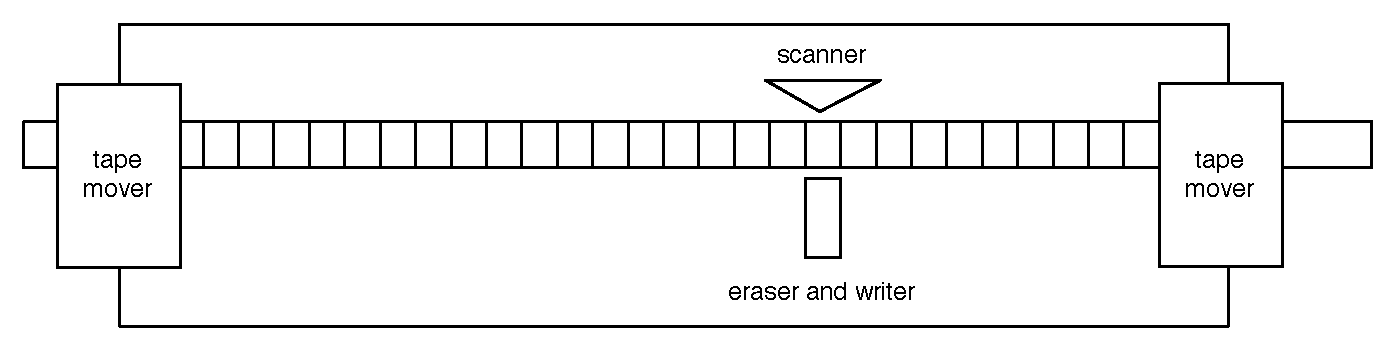
\includegraphics[width=0.9\textwidth]{turingmachine}
\caption{A Turing machine.}
\label{fig:machine}
\end{figure}


\begin{figure}
\centering
\subbottom[Turing Machine 1\label{fig:tm:tm1}]{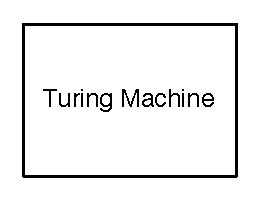
\includegraphics[width=0.2\textwidth]{block}}
\subbottom[Turing Machine 2\label{fig:tm:tm2}]{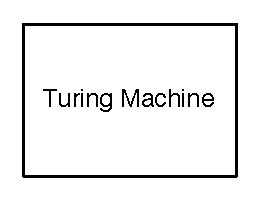
\includegraphics[width=0.2\textwidth]{block}}
\subbottom[Turing Machine 3\label{fig:tm:tm3}]{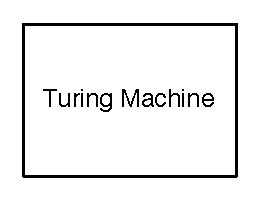
\includegraphics[width=0.2\textwidth]{block}}
\subbottom[Turing Machine 4\label{fig:tm:tm4}]{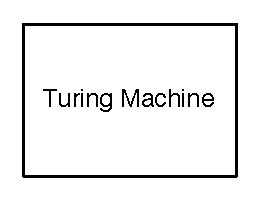
\includegraphics[width=0.2\textwidth]{block}}
\caption{Plots of four Turing machines}
\label{fig:tm}
\end{figure}




\section{Packages}
These packages might be helpful for writing your thesis:

\begin{description}
	\item[\texttt{caption}] to adjust the look of your captions
	\item[\texttt{glossaries}] for creating glossaries (also list of symbols)
	\item[\texttt{makeidx}] for indexes and the back of your document
	\item[\texttt{algorithm, algorithmicx, algpseudocode}] for adding algorithms to your document
\end{description}
%% ----------------------------------------------------------------
\thesisappendix
\thesisbib
\begin{appendices}
	% !TEX root = ../Thesis.tex
\chapter{Appendix} 
\end{appendices}
%% ----------------------------------------------------------------
\thesisback
\chapter[Declaration on Scientific Integrity]{Declaration on Scientific Integrity\\Erklärung zur wissenschaftlichen Redlichkeit}
\label{DeclarationOfAuthorship}

includes Declaration on Plagiarism and Fraud \\
beinhaltet Erklärung zu Plagiat und Betrug \vspace{1cm}

\formlabel{Author}{Autor}
\authorsint

\formlabel{Matriculation number}{Matrikelnummer}
\immatriculnrint

\formlabel{Title of work}{Titel der Arbeit}
\titleint

\formlabel{Type of work}{Typ der Arbeit}
\thesistypeint

\formlabel{Declaration}{Erklärung}
I hereby declare that this submission is my own work and that I have fully acknowledged the assistance received in completing this work and that it contains no material that has not been formally acknowledged. 
I have mentioned all source materials used and have cited these in accordance with recognised scientific rules.

\vspace{0.3cm}

Hiermit erkläre ich, dass mir bei der Abfassung dieser Arbeit nur die darin angegebene 
Hilfe zuteil wurde und dass ich sie nur mit den in der Arbeit angegebenen Hilfsmitteln 
verfasst habe. Ich habe sämtliche verwendeten Quellen erwähnt und gemäss anerkannten wissenschaftlichen Regeln zitiert. 


\vspace*{0.5cm}

Basel, \dateint
\vspace*{0.25cm}

\begin{flushright}
\rule{75mm}{0.4pt} \\
\formlabel{Signature}{Unterschrift}
\end{flushright}

%% ----------------------------------------------------------------
\end{document}
%% ----------------------------------------------------------------
